\chapter{Combinatorics}
\section{Basics}
\subsection{Considerations}
\begin{enumerate}
\item Does \textbf{order} matter?
\item Are the objects \textbf{repeatable}?
\item Are the objects partially \textbf{duplicated}?
\end{enumerate}}
If order does not matter, you can pre-set the order. 
\subsection{Basic Formula}
\begin{eqnarray*}
&& {n \choose k} = \frac{n!}{k!(n-k)!} \\
&& {n \choose k} = {n \choose n-k} \\
&& {n\choose k} = {n-1\choose k} + {n-1 \choose k-1}
\end{eqnarray*}

\subsection{N objects, K Ceils}
$$
x_1 + x_2 + x_3 = 10
$$
is equivalent to
$$
*****|**|***
$$

, notice that $*$ are duplicated.
\\
then the formula is:
$$
{n+r \choose r}
$$

,where $r=k-1$. 
\\
The meaning is to choose $r$ objects from $n+r$ objects to become the $|$.

\subsection{N objects, K types} \label{N_objects_K_types}
What is the number of permutation of $N$ objects with $K$ different types:
$$
ret = \frac{A_N^N}{\prod_{i=1}^K{A_{sz(i)}^{sz(i)}}}
$$

\subsection{Inclusion–Exclusion Principle}
\begin{figure}[hbtp]
\centering
\subfloat{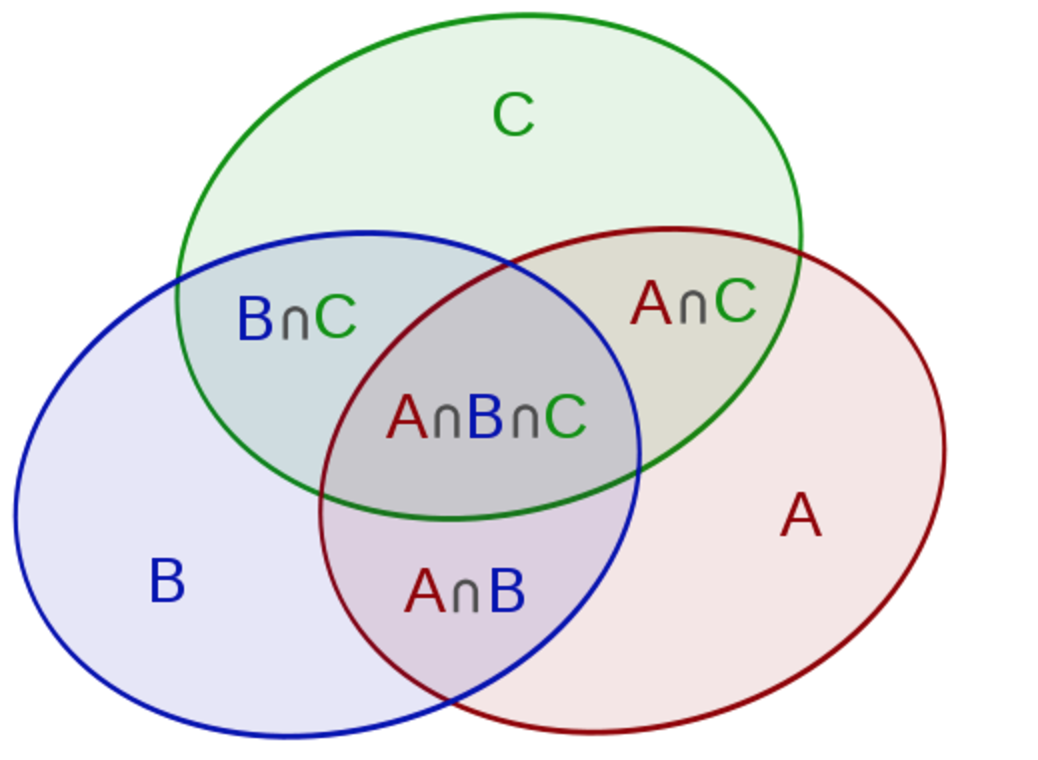
\includegraphics[scale=0.50]{500px-Inclusion-exclusion}}
\caption{Inclusion–exclusion principl}
\label{fig:500px-Inclusion-exclusion}
\end{figure}
\begin{eqnarray*}
|A \cup B \cup C| = |A| + |B| + |C| \\ - |A \cap B| - |A \cap C| - |B \cap C| \\ + |A \cap B \cap C|
\end{eqnarray*}
Generally,
$$
\Biggl|\bigcup_{i=1}^n A_i\Biggr| = \sum_{k = 1}^{n} (-1)^{k+1} \left( \sum_{1 \leq i_{1} < \cdots < i_{k} \leq n} \left| A_{i_{1}} \cap \cdots \cap A_{i_{k}} \right| \right)
$$
\section{Combinations with Duplicated Objects}
Determine the number of combinations of 10 letters (order does not matter) that can be formed from 3A, 4B, 5C. 

\subsection{Basic Solution}
If there are no restrictions on the number of any of the letter, it is ${10+2 \choose 2}$; then we get the universal set, 
$$
|U|={10+2 \choose 2}
$$

Let $P_A$ be the set that a 10-combination has more than 3A. $P_B$...4B. $P_C$...5C. 

The result is:
\begin{eqnarray*}
&& |3A \cap 4B \cap 5C| = \\
&& |U| - sum(|P_i|) + sum(|P_i \cap P_j|) - sum(|P_i \cap P_j \cap
P_k|)
\end{eqnarray*}

To calculate $|P_i|$, take $|P_1|$ as an example. \textbf{Pre-set} 4A -- if we take any one of these 10-combinations in $P_1$ and remove 4A we are left with a 6-combination with unlimited on the numbers of letters; thus,
$$
|P_1|={6+2 \choose 2}
$$

Similarly, we can get $P_2, P_3$.

To calculate $|P_i \cap P_j}|$, take $|P_1 \cap P_2|$ as an example. \textbf{Pre-set} 4A and 5B; thus,
$$
|P_1 \cap P_2| = {1+2 \choose 2}
$$

Similarly, we can get other $|P_i \cap P_j|$.

Similarly, we can get other $|P_i \cap P_j \cap P_k|$.
\subsection{Algebra Solution}
The number of 10-combinations that can be made from 3A, 4B, 5C is found from the coefficient of $x^{10}$ in the expansion of:
$$
(1+x+x^2+x^3)(1+x+x^2+x^3+x^4)(1+x+x^2+x^3+x^4+x^5)
$$

And we know:
\begin{eqnarray*}
1+x+x^2+x^3         = (1-x^4)/(1-x)  \\
1+x+x^2+x^3+x^4     = (1-x^5)/(1-x)  \\
1+x+x^2+x^3+x^4+x^5 = (1-x^6)/(1-x)  \\
\end{eqnarray*}


We expand the formula, although the  naive way of getting the coefficient of $x^{10}$ is tedious. 
